
\chapter{Introduction and Background}
\label{cha:introduction}

\epigraph{\textit{Remember that all models are wrong; the practical
    question is how wrong do they have to be to not be
    useful.}}{George Box (1987)}

\section{Motivation}
\label{sec:motivation}

Robotic planning algorithms have been widely successful in computing
feasible and optimal plans, or sequence of decisions, for tasks
involving robots operating in known environments or under known
conditions~\cite{DBLP:books/cu/L2006}. A large part of this success
can be attributed to principled algorithms that effectively
``search'' the space of all plans by exploiting the known
structure in the form of dynamical models to quickly compute the
solution. For example in the field of robot motion planning, there
have been various developments in designing planning algorithms that
exploit forward models to effectively discretize the state space into
a graph and compute a feasible plan using graph search
techniques~\cite{DBLP:books/daglib/0068760}. This enables planning
algorithms to guarantee task 
completeness, which is a requirement on the solution plan to complete
the task, and be efficient in the amount of computational resources
needed to find the solution.

However for robots to operate in unstructured environments such as
homes, offices and disaster sites, planning algorithms have to
reason about how to deal with the lack of complete knowledge of the
environment while ensuring task completeness. To retain their
effectiveness, these planning algorithms will have to utilize partial
knowledge of the environment and the task in the form of simplified
and \textit{inaccurate} dynamical models.
Naively using these inaccurate dynamical models for planning
can result in highly suboptimal plans and in some cases, plans that do
not complete the task during execution. An example of such behavior is
shown in Figure~\ref{fig:intro-example}. In this example, a robotic arm is
performing a pick-and-place task while avoiding collision with an
obstacle. In the first scenario (the first three figures from the left
in Figure~\ref{fig:intro-example},) the arm is interacting with a
light object whose mass is accurately captured by the dynamical model
used by the planner. This results in a computed trajectory for the
arm that grasps the object, lifts it above the obstacle and takes it
to the goal location. While this scenario has highlighted the
effectiveness of the planning algorithm to complete the task when
given access to an accurate dynamical model, consider the second
scenario (the last figure on the right in
Figure~\ref{fig:intro-example}) where the arm is interacting with a
heavy object which is modeled as a light object by the dynamical
model. Since the model is same as before, the planner computes the
same trajectory which lifts the object above the obstacle. However,
while executing the trajectory the arm cannot lift the heavy object and
cannot command the joint torques required because they are beyond the
arm's capabilities. Thus, the computed plan is not successful in
completing the task.
\begin{figure*}[t]
  \centering
  \begin{subfigure}{0.24\linewidth}
    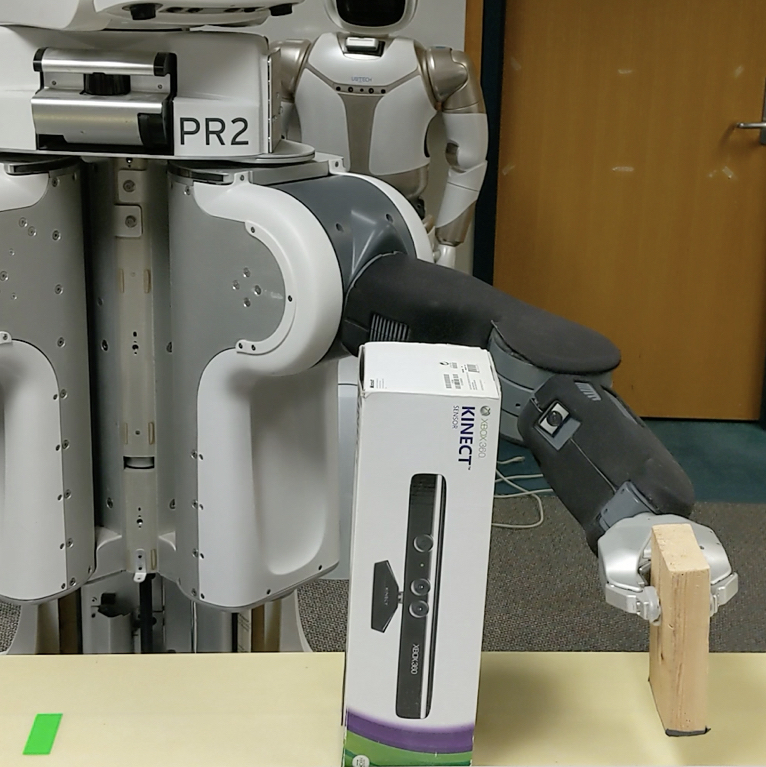
\includegraphics[width=\linewidth]{figures/cmax/pr2_pick_place_light_1_annotated.jpeg}
  \end{subfigure}
  \begin{subfigure}{0.24\linewidth}
    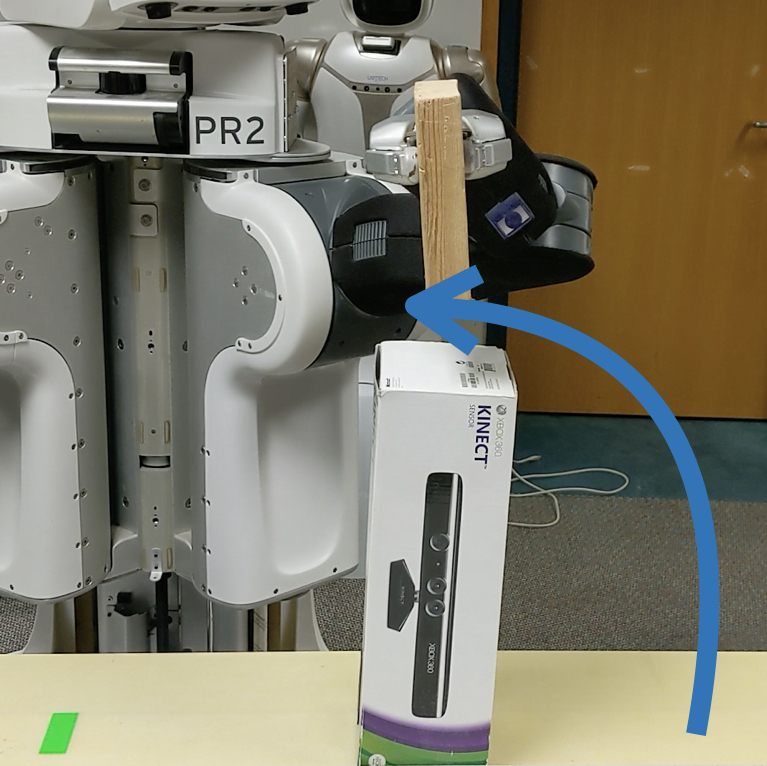
\includegraphics[width=\linewidth]{figures/cmax/pr2_pick_place_light_2_annotated.jpeg}
  \end{subfigure}
  \begin{subfigure}{0.24\linewidth}
    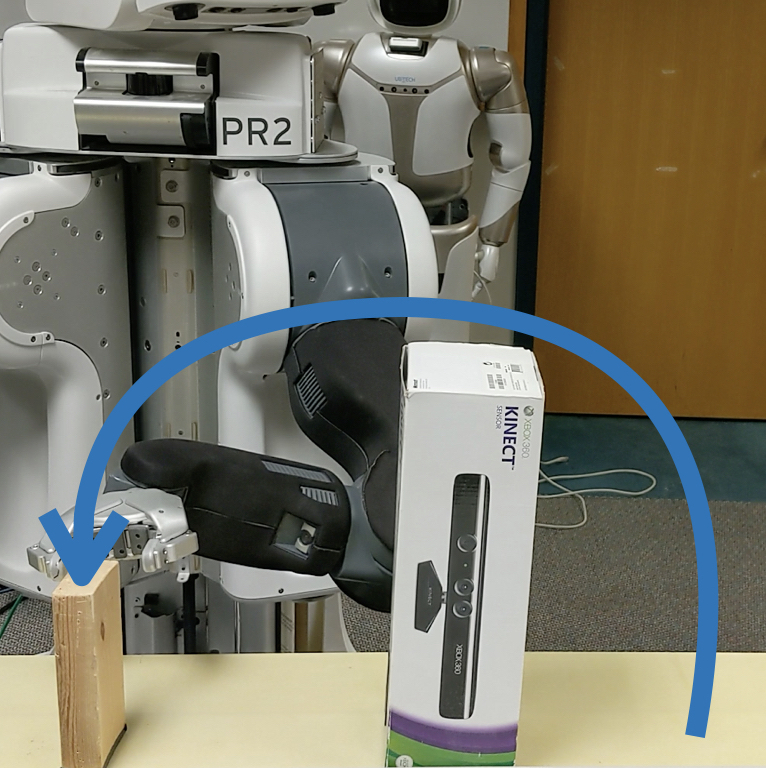
\includegraphics[width=\linewidth]{figures/cmax/pr2_pick_place_light_3_annotated.jpeg}
  \end{subfigure}
  \begin{subfigure}{0.24\linewidth}
    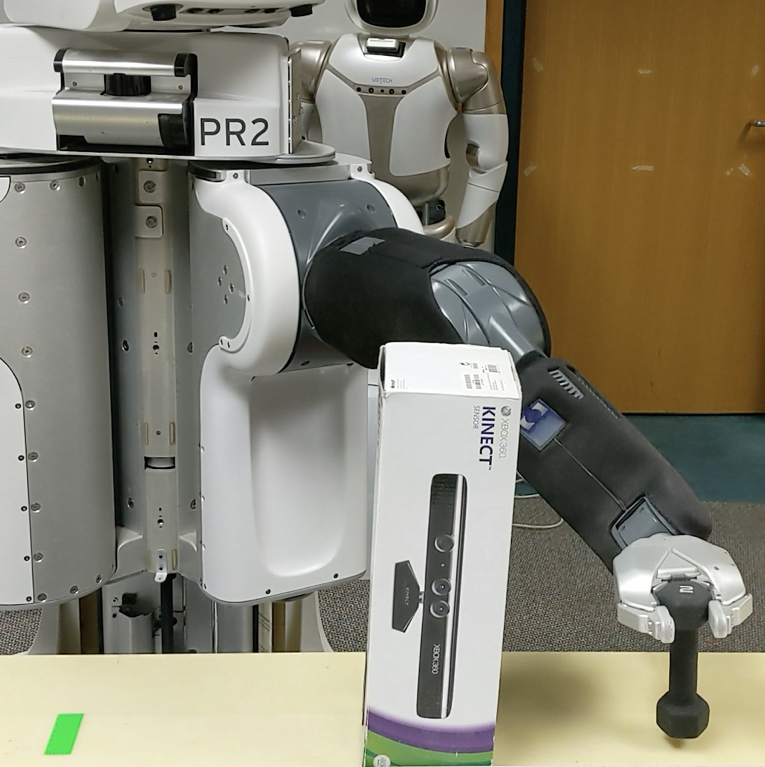
\includegraphics[width=\linewidth]{figures/cmax/pr2_pick_place_heavy_1_annotated.jpeg}
  \end{subfigure}
  \caption{A robotic arm picking an object from its start location and
  placing it at a goal location while avoiding collision with the
  intermediate obstacle during motion. The first three (from left)
  figures show an execution with a light object (wooden block) and a
  plan (blue trajectory) computed
  using an accurate dynamical model which captures the weight of the
  object correctly. The last figure (rightmost) shows an instance of
  the same task but with a heavy object (black dumbbell) and same
  dynamical model as before which models the object as light. This
  results in the planner computing the same plan as before, which the
  robot cannot execute as lifting the heavy object requires joint
  torques that are beyond the robot's capabilities. Thus, the plan is
  not task complete.}
  \label{fig:intro-example}
\end{figure*}
The above example highlights the ineffectiveness of naively using
these inaccurate models for planning. This ineffectiveness can be
tackled broadly in two directions: updating either the dynamical
model or the behavior of the planner, using the accumulated
experience during execution.

The former direction of using online
experience to update existing dynamical models or learning new
dynamical models from scratch has been explored in the Reinforcement
Learning (RL) framework. This framework enables autonomous agents,
such as robots, to learn how to operate in an unknown environment by
interacting with it and compute an optimal plan that minimizes total
cost~\cite{sutton1998introduction}. With partial or no prior knowledge
about the environment, the agent needs to explore to discover low cost
actions or regions where dynamics are inaccurately modeled. The
exploration strategies leveraged by these agents require a large
amount of interactions with the environment before we can compute
plans that guarantee task completeness. This is a major reason why RL,
despite being a very general framework, has mostly seen success in
domains where we can afford to collect large amounts of interactions
with little effort: video games and simulations.

Most methods in the RL framework can be categorized as either model-based
or model-free (Figure~\ref{fig:dyna}). As the name suggests, model-based methods rely on
using a model as input to a planning procedure to compute the solution
plan for a given task. These methods use the experience gained online
during execution to update the dynamics of the model and replan to
compute a new solution plan~\cite{DBLP:journals/sigart/Sutton91}. In
contrast, model-free methods directly 
use the accumulated experience to compute an updated solution plan
without ever using a dynamical model. These methods utilize the
experience to estimate value functions, which are esentially
cost-to-go estimates, and compute a plan using the estimated
values. Both methods have advantages and disadvantages. Model-based
methods relatively require fewer amounts of experience to compute a
plan of the same quality as the plan computed by a model-free
method. On the other hand, model-free methods are not affected by the biases
inherent in the design of the model.

\begin{figure}[t]
  \centering
  \includegraphics[width=0.5\linewidth]{Figures/intro/dyna.pdf}
  \caption{Operation of Model-based (blue) and Model-Free RL (red) methods
    while executing in unknown environments and collecting
    experience to complete a task. Figure inspired from Dyna~\cite{DBLP:journals/sigart/Sutton91}}
  \label{fig:dyna}
\end{figure}

In contrast, the latter direction of updating the behavior of the
planner using online experience has not been explored as extensively
in past literature. Interestingly, this direction has been explored by
the practitioner for quite some time. As motivated earlier, in most
robotic tasks we seldom have access to accurate dynamical models and
the models we use for planning are often inaccurate. Robotics
engineers and practitioners have been dealing with these inaccuracies
by modifying how the planner uses the inaccurate model rather than
updating the model to improve its accuracy. As an example, consider
the task of planning footsteps of a mobile quadruped robot over
partially unknown terrain as shown in Figure~\ref{fig:zucker} taken
from \cite{DBLP:journals/ijrr/ZuckerRSCBAK11}. The
unknown part of the terrain is annotated in the figure (red oval.) To
ensure that the planner does not compute footstep trajectory that goes
through this region, a simple
hack that the practitioner does is to inflate the cost of any
state-action pair that takes the robot into this region. This results
in biasing the planner away from this region thereby updating its
behavior. There are several other example applications where the
practitioner deals with inaccurate modeling by simply updating the
behavior of the planner. While this direction has been explored by the
practitioner, there is very little prior work that has studied this
direction from a theoretical point of view aiming to understand the
assumptions required to guarantee task completeness, and a systematic
study to analyze its empirical performance in practice. Our thesis
aims to fill this gap and develop a better understanding when, where
and how these methods work well in practice.

\section{Thesis Goal and Contributions}
\label{sec:thes-goal-contr}

While most existing works have presented and studied approaches that
use the experience from executions to update the dynamics of the
inaccurate model, one can argue that this is wasteful if we are interested in
completing the task and not in modeling the dynamics
accurately. Furthermore, robots operating in the real world have
operating constraints that require them to quickly adapt to
new scenarios and not spend hours acquiring experience to learn true
dynamics. In such spirit, our main focus in this thesis is to argue that by updating the
behavior of the planner and not the dynamics of the model, we can
leverage simplified and potentially inaccurate models and
significantly reduce the amount of real-world experience needed to
provably guarantee that the robot completes the task.

\begin{figure}[t]
  \centering
  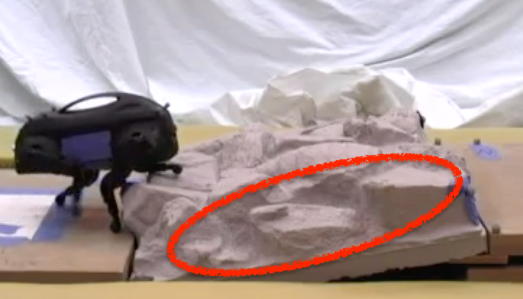
\includegraphics[width=0.5\linewidth]{Figures/intro/zucker}
  \caption{A practitioner's approach to dealing with inaccuracies in
    dynamical models used for planning. In this example, the robot is
    planning a footstep trajectory along the partially unknown terrain
  to reach the other side. The planner has access to a model of the
  terrain which is inaccurate in the regions marked by red oval. To
  ensure that the planner does not compute any trajectory going
  through the red oval region, practitioners typically inflate the
  cost of any action executed within the region or any action that
  takes the robot into this region. This results in biasing the
  planner away from this region thereby updating its behavior. Figure
  taken from \cite{DBLP:journals/ijrr/ZuckerRSCBAK11} and the red oval
  region depicted is an example used for emphasis.}
\label{fig:zucker}
\end{figure}

We support this argument by presenting two methods that update the
behavior of the planner and do not require any updates to the dynamics
of the inaccurate model used for planning.  Both methods come with
provable guarantees on completing the task under assumptions on the
accuracy of the model. In addition to these methods, we also emphasize
the importance of using model-based planning
by analyzing the sample complexity (or the amount of experience
needed) of exploration techniques used in model-free RL methods. Our
analysis shows that undirected global exploration techniques popularly
used in model-free RL methods can result in large sample complexity
requirements that cannot be realized in practice on a robot.

The primary contributions of this thesis can be detailed as follows.

\subsection{Sample Complexity of Exploration in Model-Free Policy
  Search}
\label{sec:sample-compl-expl}
We analyze the sample complexity of exploration techniques in
  model-free RL methods. This analysis is presented by viewing model-free policy
  search methods through the lens of derivative-free optimization (DFO)
  and computing upper bounds on the number of samples
  required to compute a $\epsilon$-suboptimal policy. We present a DFO
  point of view for methods that involve either exploration in action
  space or exploration in policy space, and present trade-offs between
  both styles of exploration in terms of the dimensionality of the
  policy parameter space, and the horizon length of the task. This
  analysis is presented in Chapter~\ref{cha:sample-compl-expl} of the  
  thesis and is also presented in our paper~\cite{aistats19}. In addition
  to contrasting exploration in policy space vs action space, this
  work also emphasizes the large sample complexity required by
  model-free methods, which cannot be realized in practice on a robot.
  
\subsection{Planning and Execution using Inaccurate Models}
\label{sec:plann-exec-using}
  We present the first systematic effort to understand methods
  that use online experience from executions to update the behavior of
  the planner and not update the dynamics of the model. Thus, these
  methods can make progress towards completing the task despite using
  a potentially inaccurate model. One can construct cases where if the
  model is highly inaccurate (e.g. a model that predicts a humanoid
  falling down for any action and failing to complete the task of
  moving forward,) then such a method cannot be expected to finish the
  task. Hence, we study the assumptions required on the accuracy of
  the model used for planning that ensures task completeness without
  requiring any updates to the dynamics of the model. Furthermore, we
  frame our problem in the purely online setting where the experience
  gathered by the robot is along a single trajectory without any
  access to resets. We believe that this setting is realistic and has
  challenges that these methods are uniquely positioned to tackle.

  We propose \cmax{}, an approach that guarantees that the robot
  completes the task using the inaccurate model without any resets and
  without requiring any updates to the dynamics of the model. This is
  achieved by biasing the planner away from transitions whose dynamics
  are discovered to be inaccurately modeled during online
  execution. On the theoretical side, we establish provable guarantees
  on task completeness under assumptions on the accuracy of the model
  used for planning. Empirically, we show that \cmax{} outperforms
  state-of-the-art model-free and model-based RL methods in terms of
  the number of executions taken to complete the task. Crucially,
  \cmax{} exhibits goal-driven behavior which enables it to focus on
  completing the task as quickly as possible and not waste executions  
  learning the true dynamics. This method is explained in detail in
  Chapter~\ref{cha:plann-exec} and is also presented in our
  paper~\cite{cmax}.

\subsection{Leveraging Experience in Planning and Execution using
  Inaccurate Models}
\label{sec:lever-exper-plann}
  
While a robot using \cmax{} is provably guaranteed to complete
  the task, it requires strong assumptions on the accuracy of the
  model that are often not realized in practice and hard to verify
  prior to execution. In addition for repetitive tasks, \cmax{} fails
  to improve the quality of the solution over repetitions of the same
  task as it does not leverage previously discovered inaccurately
  modeled transitions. This is remedied by our second approach
  \cmaxpp{} that leverages experience from past executions to improve
  the quality of solution over repetitions of the same
  task. Crucially, unlike \cmax{}, \cmaxpp{} can compute solution
  plans that contain previously discovered inaccurately modeled
  transitions. \cmaxpp{} achieves this by integrating model-free value
  learning using acquired experience with model-based planning using
  the inaccurate model. As a consequence of this in addition to
  completeness, \cmaxpp{} also guarantees asymptotic convergence to
  the optimal path cost as the number of repetitions increases. These
  guarantees of \cmaxpp{} are established under assumptions on the
  accuracy of the model that are much more relaxed compared to the
  assumptions required by \cmax{}. Importantly, like \cmax{},
  \cmaxpp{} never updates the dynamics of the model. This method is
  explained in detail in Chapter~\ref{cha:lever-exper} and is also 
  presented in our paper~\cite{cmaxpp}.

\section{Background}
\label{sec:background}

In this section, we provide background knowledge with the aim of
introducing classical techniques
that we will use throughout this thesis. Each chapter of this thesis
is self-contained and has detailed definitions that are more tailored
to the specific problem tackled in each chapter.

\subsection{Fundamentals of Markov Decision Processes}
\label{sec:fund-mark-decis}

In this thesis, we will primarily deal with finite horizon problems
where the objective is for an agent to minimize cumulative cost incurred over a
horizon of finite length. This is typically formulated as a finite horizon Markov
Decision Process (MDP)~\cite{bellman} that is represented as
$(\statespace, \actionspace, P, c, H)$ where $\statespace$ is the set
of states that the agent can be in, $\actionspace$ is the set of
actions that the agent can execute, $P$ is the transition dynamics
such that for any $s_t \in \statespace$, $s_{t+1} \in \statespace$,
$a_t \in \actionspace$, $P(s_{t+1}|s_t, a_t)$ is the probability of
transitioning to state $s_{t+1}$ from state $s_t$ by taking action
$a_t$, $c$ is the cost function such that for any transition $(s_t,
a_t)$, $c(s_t, a_t)$ is the cost incurred for that transition, and $H
\in \mathbb{N}^+$ is the length of the horizon. Typically, this
formulation also has a discounting factor $\gamma$ and a initial state
distribution $\rho$. In this thesis, we consider the non-discounted
setting where $\gamma = 1$ and a fixed initial state $s_0$ that is
known (thus, $\rho$ is a delta distribution on $s_0$.)

A deterministic policy $\pi: \statespace \rightarrow \actionspace$
maps from a state to an action. Given $\pi$ and a time step $t$, we can define the 
cost-to-go or value estimate $V_\pi^t(s)$ as follows:
\begin{equation}
  \label{eq:3}
  V_\pi^t(s) = \mathbb{E}\left[ \sum_{i=t}^H c(s_i, a_i) | a_i =
    \pi(s_i), s_{i+1} \sim P_{s_i, a_i}, s_t = s \right]
\end{equation}
where $P_{s_i, a_i} = P(\cdot|s_i, a_i)$ is a distribution over the
next state.

Similarly, we can also define the state-action value estimate
$Q_\pi^t(s, a)$ as follows:
\begin{equation}
  \label{eq:4}
  Q_\pi^t(s, a) = c(s, a) + \mathbb{E}_{s' \sim P_{s,a}}[V_\pi^{t+1}(s')]
\end{equation}

The objective function $J(\pi)$ is defined as
\begin{equation}
  \label{eq:6}
  J(\pi) = V_\pi^0(s_0)
\end{equation}
and the goal is to find a policy from a given policy set $\Pi$ that
minimizes the above objective function.

If the cost function and the transition dynamics is known, then one
can compute the optimal policy using Dynamic Programming (DP.) Denote
the optimal policy using $\pi^*$. Define $Q_{\pi^*}^{H-1}(s, a) = c(s,
a)$, we perform DP as follows: Starting from $t = H-2$ until $t = 1$
we iteratively do
\begin{align}
%  \label{eq:7}
  V_{\pi^*}^t(s) &= \max_{a \in \actionspace} Q_{\pi^*}^t(s, a) \\
  Q_{\pi^*}^{t-1}(s, a) &= c(s, a) + \mathbb{E}_{s' \sim P_{s, a}}[V_{\pi^*}^t(s')]
\end{align}
Given $Q_{\pi^*}^t$ we can compute the optimal action at time step $t$
and state $s_t$ 
as $\min_{a \in \actionspace} Q_{\pi^*}^t(s_t, a)$. The above
iterative process is called as Value Iteration. This iterative
procedures is derived by observing that the value function of the
optimal policy satisfies the following fixed point equation
\begin{equation}
  \label{eq:8}
  V_{\pi^*}^t(s) = \min_{a \in \actionspace} \left( c(s, a) + \mathbb{E}_{s'
  \sim P_{s,a}}[V_{\pi^*}^{t+1}(s')]\right)
\end{equation}
The above equation is known as the Bellman optimality condition.

\subsection{Deterministic Shortest Path Problem}
\label{sec:determ-short-path}

The shortest path problem is to find among all paths that start at a
given state and end at a goal state, a path has the minimum cost; this
is also called a shortest path~\cite{bertsekas1995neuro}. This can be instantiated as a markov
decision process represented using the tuple $(\statespace,
\actionspace, \goalspace, f, c)$ where $\goalspace \subseteq
\statespace$ is the set of goal states, and $f:\statespace \times
\actionspace \rightarrow \statespace$ is a deterministic
dynamics function that determines the successor state $s_{t+1}$ of a
transition $(s_t, a_t)$ as $f(s_t, a_t)$. The goal states in
$\goalspace$ are cost-free termination states, i.e. $f(g, a) = g$, $c(g,
a) = 0$ for
all $g \in \goalspace$ and any action $a \in \actionspace$. We also
assume that the cost of any transition starting from a non-goal state
is positive, i.e. $c(s, a) > 0$ for all $s \in \statespace \setminus
\goalspace$ and $a \in \actionspace$.

We are interested in problems where reaching the termination state is
inevitable, at least under an optimal policy. Thus, the essence of the
problem is how to reach a goal state with minimum cost. In the
shortest path problem setting, we use $V(s)$ to denote the cost-to-go
(or value) estimate of any state $s \in \statespace$ and $V^*(s)$ to
denote the optimal cost-to-go (or value.) From the Bellman optimality
condition we know
\begin{equation}
  \label{eq:9}
  V^*(s) = \min_{a \in \actionspace}\left( c(s, a) + V^*(f(s, a)) \right)
\end{equation}
A value estimate $V$ is called admissible if underestimates the
optimal value at all states, i.e. $V(s) \leq V^*(s)$ for all $s \in
\statespace$. Furthermore, $V$ is called consistent if it satisfies
the condition that for any state-action pair $(s, a)$, $s \notin
\goalspace$, $V(s) \leq c(s, a) + V(f(s, a))$ and $V(g) = 0$ for all
$g \in \goalspace$.
A typical assumption made in all shortest path problems is that there
exists at least one path from each state $s \in \statespace$ to one of
the goal states in $\goalspace$. This ensures that the optimal value
for any state is finite.

\subsection{Real-time Heuristic Search}
\label{sec:real-time-heuristic-1}

A traditional way to solve the shortest path problem is to search the
graph constructed using a mental model of the world, and then
subsequently execute the resulting plan (or follow the computed path.)
Thus, planning and execution are completely separated. An alternative
way of solving this problem is to search online by interleaving
planning and execution which results in several advantages with the
major advantage being drastic reductions in planning time. This is
achieved by performing search locally until a fixed horizon (or until
a fixed number of states are expanded,) and then execute the best
action for the current state. After the execution, planning is
performed once again to find the next best action. This can decrease
the time used for planning as we are not planning all the way to the
goal. Another significant advantage is when the mental model of the
world is inaccurate, these methods enable the agent to update its
model and ensure future replanning results in more optimal paths.

Since the future consequences of executed actions are unknown,
interleaving planning and execution can result in slight overhead in
terms of the number of actions executed but this is often a much
smaller overhead compared to the reduced planning time. Real-time
search methods are methods that interleave planning and execution by
searching forward from the current state of the agent. Most
importantly, real-time heuristic search methods can satisfy hard
real-time requirements in large state spaces since the sizes of their
local search spaces are independent of the sizes
of the state spaces and can thus remain small.

\subsubsection{LRTA*}
\label{sec:lrta}

In this thesis, we will focus on Learning real-time A* (LRTA*) real-time search methods
that are real-time search methods that associate information with the
states to prevent cycling. These methods are promising for
interleaving planning and execution as they are efficient
domain-independent search methods that allow fine-grained control over
how much planning is allowed between executions, use heuristic
knowledge to guide planning, and improve their performance over time
as they solve similar planning tasks. LRTA* operates on deterministic
domains only.

\begin{algorithm}[t]
  \caption{LRTA* with Lookahead $1$~\cite{DBLP:journals/ai/Korf90}}
  \begin{algorithmic}[1]
    \State $s \leftarrow s_0$
    \While{$s \notin \goalspace$}
    \State Compute action $a = \argmin_{a \in \actionspace} \left( c(s, a) +
      V(f(s, a)) \right)$
    \State Update $V(s) \leftarrow \min\left( V(s), c(s, a) + V(f(s,
      a)) \right)$
    \State Execute action $a$ and update $s \leftarrow f(s, a)$
    \EndWhile
  \end{algorithmic}
  \label{alg:lrta}
\end{algorithm}

Algorithm~\ref{alg:lrta} presents the LRTA* algorithm for a lookahead
or search horizon of $1$. At each time step, the algorithm looks one
action execution ahead and always greedily chooses the action that
leads to a successor state with the minimum sum of cost of
transitioning into the successor state and the value estimate of the
successor state. Furthermore unlike classical real-time search
methods, LRTA* also updates the value estimates of the current state
to reflect the updated estimate of the best path to the goal so that
future replanning is more efficient. The planning time of LRTA*
between executions is linear in the number of actions. If the size of
action space is independent of the size of state space, then the
planning time is independent of the size of state space which is a
major improvement over offline planning methods whose computational
complexity is at most the size of the state space.

LRTA* can be viewed as a form of asynchronous incremental dynamic
programming method~\cite{DBLP:journals/ai/BartoBS95}. It can be shown
that LRTA* is guaranteed to reach a goal state in a finite number of
executions and if we reset to the start state after reaching the goal
state, then the value estimates eventually converge to the optimal
value function~\cite{DBLP:journals/ai/Korf90}. These guarantees hold
under the assumption that the initial value estimates that we start
with are admissible and consistent. These assumptions are very similar
to the traditional definitions of admissible and consistent heuristic
values for A* search. Note that zero-initialized value estimates are
both admissible and consistent.

\subsubsection{RTAA*}
\label{sec:rtaa}

Real-time Adaptive A* (RTAA*) proposed
in~\cite{DBLP:conf/atal/KoenigL06} is similar to LRTA*
(Algorithm~\ref{alg:rtaa}). They only 
differ in the way they update the
value estimates at each time step. To understand this better, let us
look at how LRTA* updates value estimates. LRTA* replaces the value
estimate of each expanded state with the sum of costs of from the
state to a generated but unexpanded state $s$ (leaf node in the search
tree) and the value estimate of state $s$, minimized over all
generated but unexpanded states (all leaf nodes of the search tree.)
If we denote $V$ as the value estimates after all the value
updates then the LRTA* updates satisfy the following system of
equations for all expanded states $s$:
\begin{equation}
  \label{eq:10}
  V(s) = \min_{a \in \actionspace}\left( c(s, a) + V(f(s, a)) \right)
\end{equation}

\begin{algorithm}[t]
  \caption{RTAA* with lookahead $K \geq 1$~\cite{DBLP:conf/atal/KoenigL06}}
  \begin{algorithmic}[1]
    \State $s \leftarrow s_0$
    \While{$s \notin \goalspace$}
    \State Construct a search tree at $s$ until $K$ expansions
    \State Estimate $\bar{s}$ as the leaf node with the least $g + V$
    estimate among all leaf nodes
    \For{all expanded states $s'$}
    \State Update $V(s') \leftarrow g(\bar{s}) + V(\bar{s}) - g(s')$
    \EndFor
    \State Compute action $a$ as the first action on the path from
    state $s$ to state $\bar{s}$ in the search tree
    \State Execute action $a$ and update $s \leftarrow f(s, a)$
    \EndWhile
  \end{algorithmic}
  \label{alg:rtaa}
\end{algorithm}

On the other hand, RTAA* constructs a search tree very similar to
LRTA* (the number of states expanded is equal to the lookahead) but
updates the value estimates for all expanded states $s$ as follows:
\begin{equation}
  \label{eq:11}
  V(s) = g(\bar{s}) + V(\bar{s}) - g(s)
\end{equation}
where $g(s)$ encodes the cost-to-come from the root of the search tree
to the state $s$ (i.e. sum of costs of all transitions on the path
from root to state $s$,) and $\bar{s}$ is the state corresponding to
the leaf node with the least sum of $g$ and $V$ among all leaf nodes
in the search tree. In other words, $\bar{s}$ is the state that was
about to be expanded just before the search was terminated. One can
show that LRTA* and RTAA* updates are exactly the same when the
lookahead is $1$. But when the lookahead is greater than $1$, these
updates differ. More specifically, LRTA* updates tend to be more
informed or reflect the optimal cost-to-go better when compared to
RTAA* updates. However, it takes LRTA* more time to update the value
estimates and is difficult to implement. This is because LRTA*
performs one search to determine the local search space and a second
search to determine how to update the value estimates since it is
unable to use the results from the first search for this
purpose. Thus, there is a trade-off between the total search time and
cost of the resulting path. In practice, for lookaheads greater than
$1$, RTAA* tends to compute solution paths that have higher costs
compared to LRTA* but the time taken for planning before each execution is
significantly less in RTAA* compared to LRTA*. This makes RTAA*
desirable in applications where planning is slow but actions can be
executed fast and there is a very strict time limit per search episode.

\subsection{Local Function Approximation Methods}
\label{sec:local-funct-appr-1}

The goal of function approximation methods is to capture the
underlying relationship between input and output data. A typical
approach is to use all the training data to fit a global model that
predicts the output given the input throughout the input space. The
hope is that this approximation predicts output values that are close to the
true output values of the original function. A major disadvantage of
these global function approximation methods is that in many cases,
there exists no parameter values that provide a sufficiently good
approximation. Moving to a larger function approximation class with
more parameters requires a significantly larger training data which
might not be available. Furthermore, in cases where the model needs to
be updated incrementally, the computational cost of recomputing the
global function approximation is very high and potentially infeasible
on real-time systems.

An alternative to global function approximation methods are local
function approximation methods such as Locally Weighted Learning
(LWL)~\cite{DBLP:journals/air/AtkesonMS97a,
  DBLP:journals/air/AtkesonMS97}. LWL methods are 
non-parametric and prediction is computed using local functions which
use only a subset of the training data. The basic idea of LWL is for
each query point, a local model is constructed based on
neighboring training data. Each data point is associated with a
weighting factor that captures the influence of the data point in
computing the prediction for the query point. Intuitively, the closer
the data point to the query point the higher its influence. Since the
training data is directly used during prediction and there is no
pre-processing before prediction, LWL can be a very accurate and fast
incremental function approximation method.

For ease of exposition, let us consider the following regression
model
\begin{equation}
  \label{eq:12}
  y = f(\xbold) + \epsilon
\end{equation}

where $f(\xbold)$ is the unknown function that we are seeking to
approximate, $\xbold \in \mathbb{R}^d$, $y \in \mathbb{R}$ and
$\epsilon$ is zero mean noise. Given a dataset
$\buffer = \{(\xbold_i, y_i)\}_{i=1}^N$ and a query point $\xbold_q$ we can define
the following cost function,
\begin{equation}
  \label{eq:13}
  J(\beta_q) = \frac{1}{N}\sum_{i=1}^N w_i(\xbold_q)(y_i - \betabold_q^T\xbold_i)^2
\end{equation}
where $w_i$ are weights that capture the influence of the $i$-th data
point $(\xbold_i, y_i)$ on the prediction for query point $\xbold_q$, and
$\betabold_q$ is the coefficients for our linear model that is used for
prediction. The goal is to find $\betabold_q$ that minimizes the above
cost function and predict $\hat{y}_q = \betabold_q^T\xbold_q$ (Assume
that $\xbold_i, \xbold_q$ vectors have a $1$ added to account for the
offset term.) The weights $w_i(\xbold_q)$ are computed typically using
a distance metric $d(\xbold_i, \xbold_q)$ that captures relevance of
training points to the query point, and a kernel function $K(d)$ which
computes the weight given a distance value.

\subsubsection{K-Nearest Neighbor Regression}
\label{sec:k-nearest-neighbor}

A very simple LWL method is K-Nearest Neighbor (KNN) regression which
given a query point $\xbold_q$ finds the $K$ nearest neighbors in the
training data $\buffer$ using a distance metric $d(\xbold_q,
\xbold_i)$. There are several variants of this method, one of which
uniformly weights all the $K$ nearest neighbor's outputs to obtain the
prediction for the query point, i.e.
\begin{equation}
  \label{eq:14}
  \hat{y}_q = \frac{1}{K} \sum_{\xbold_i \in \buffer_K(\xbold_q)} y_i
\end{equation}
where $\buffer_K(\xbold_q)$ represents the set of size $K$ consisting
of the $K$ nearest neighbors of the query point $\xbold_q$ in
$\buffer$. Another variant, which often works well in practice, is to
weigh each neighbor by the inverse of their distance to the query
point. Intuitively, closer neighbors have a greater influence than
farther neighbors. Thus, we have
\begin{equation}
  \label{eq:15}
  \hat{y}_q = \frac{\sum_{\xbold_i \in \buffer_K(\xbold_q)} w_iy_i}{\sum_{\xbold_i \in \buffer_K(\xbold_q)} w_i}
\end{equation}
where the weight $w_i = \frac{1}{d(\xbold_q, \xbold_i)}$ is the
inverse of distance to the query point. KNN regression requires
storing all the training data in memory in the form of K-d trees which
allow very fast computation of $K$ nearest neighbors.

\subsubsection{Locally Weighted Regression}
\label{sec:locally-weight-regr}

Locally weighted regression (LWR) is a locally weighted learning
method that maintains all the training data in memory and quickly
computes the prediction for any given query point. LWR is presented in
Algorithm~\ref{alg:lwr} which is executed once for each query point
$x_q$. There are also simple extensions to the batch setting where we
want to obtain predictions for a batch of query points. The only
hyperparameter is the matrix $D$ which is usually set to a scaled
identity matrix $D = h\mathbb{I}$ where $h$ is a scalar hyperparameter
that is chosen using cross validation. LWR typically has a very high
approximation accuracy due to its local nature and has only few
hyperparameters. The disadvantage is that Algorithm~\ref{alg:lwr} has
a computational complexity of $\mathcal{O}(N^2)$ where $N$ is the size
of training data, which can be very expensive for large
datasets. Furthermore, LWR requires you to store all the training data
in memory which might be infeasible for extremely large datasets.

\begin{algorithm}[t]
  \caption{Locally Weighted Regression}
  \begin{algorithmic}[1]
    \State \textbf{Input:} Training data $\buffer = \{(\xbold_i,
    y_i)\}_{i=1}^N$, Query point $\xbold_q$
    \State Construct matrix $X$ with rows corresponding to $\hat{\xbold}_i$
    where $\hat{\xbold}_i = [\xbold_i^T 1]^T$
    \State Construct vector $\ybold$ with each element corresponding
    to $y_i$
    \State Compute diagonal weight matrix $W$ where the $i$-th
    diagonal element is given by $\exp\left( -\frac{1}{2} (\xbold_i -
      \xbold_q)^TD(\xbold_i - \xbold_q) \right)$
    \State Compute $\beta_q = (X^TWX)^{-1}X^TW\ybold$
    \State Compute prediction $\hat{y}_q = \beta_q^T\hat{\xbold_q}$
    where $\hat{\xbold_q} = [\xbold_q^T 1]^T$
  \end{algorithmic}
  \label{alg:lwr}
\end{algorithm}


%%% Local Variables:
%%% mode: latex
%%% TeX-master: "../main"
%%% End:
